\documentclass[xcolor=dvipsnames]{beamer}
\usetheme{Montpellier}
\usepackage[utf8]{inputenc}
\usepackage{amsmath}
\usepackage{amsfonts}
\usepackage{amssymb}
\usepackage{graphicx}
\author{Sahil Dhawan}
\title[Analyzing Topological Properties of 3D files]{Analyzing the Topological Properties of 3D STL Files}
%\setbeamercovered{transparent} 
%\setbeamertemplate{navigation symbols}{} 
%\logo{} 
\institute[UNC Greensboro]{University of North Carolina at Greensboro} 
\date{March 12, 2024} 

\setbeamercolor{structure}{fg=red}
    \setbeamercolor{normal text}{fg=white}
\setbeamercolor{background canvas}{bg=black}
\setbeamercolor{local structure}{fg=white}
\begin{document}

\begin{frame}
\titlepage
\end{frame}

\begin{frame}
\tableofcontents
\end{frame}

\section{Introduction}
\begin{frame}{Introduction}

\end{frame}

\subsection{Related Works}
\begin{frame}{Related Works}

\end{frame}

\section{Background}
\begin{frame}{Background}

\end{frame}

\subsection{Simplicial Homology}
\begin{frame}{Simplicial Homology}

\end{frame}

\subsection{Persistent Homology}
\begin{frame}{Persistent Homology}

\end{frame}

\subsection{Triangulation}
\begin{frame}{Triangulation}

\end{frame}

\subsection{Background on the STL Filetype}
\begin{frame}{Background on the STL Filetype}

\end{frame}

\section{Methods}
\subsection{Main Method}
\begin{frame}{Methods, Main Method}
\begin{enumerate}
\item Creating a Mesh from an STL File
\item Creating and Modifying an Alpha Complex
\item Computing a Persistence Diagram
\end{enumerate}
\end{frame}

\begin{frame}{Creating a Mesh from an STL File}

\end{frame}

\begin{frame}{Creating and Modifying an Alpha Complex}

\end{frame}

\begin{frame}{Computing a Persistence Diagram}

\end{frame}

\subsection{Implementation}
\begin{frame}[fragile]{Methods, Implementation}
\begin{enumerate}
\item Creating STL Files with FreeCAD
\item Parsing the STL File Data
\item Creating a Constrained Delaunay Triangulation with \verb"meshpy"
\item Creating and Modifying an Alpha Compplex with \verb"gudhi"
\item Filtration Construction with \verb"gudhi"
\item Persistence Diagram Construction
\end{enumerate}
\end{frame}

\begin{frame}{Creating STL Files with FreeCAD}

\end{frame}

\begin{frame}{Parsing the STL file Data}

\end{frame}

\begin{frame}{Creating a Constrained Delaunay Triangulation with meshpy}

\end{frame}

\begin{frame}{Creating and Modifying an Alpha Compplex with gudhi}

\end{frame}

\begin{frame}{Filtration Construction with gudhi}

\end{frame}

\section{Results and Discussion}
\subsection{Two Cubes with Three Pockets Moving Closer}
\begin{frame}{Two Cubes with Three Pockets Moving Closer}

\end{frame}

\subsection{Cube with Equilateral Triangle Hole}
\begin{frame}{Cube with Equilateral Triangle Hole}

\end{frame}

\subsection{Rectangular Prism Ring with Cut}
\begin{frame}{Rectangular Prism Ring with Cut}
\begin{table}[H]
\begin{tabular}{cccccc}
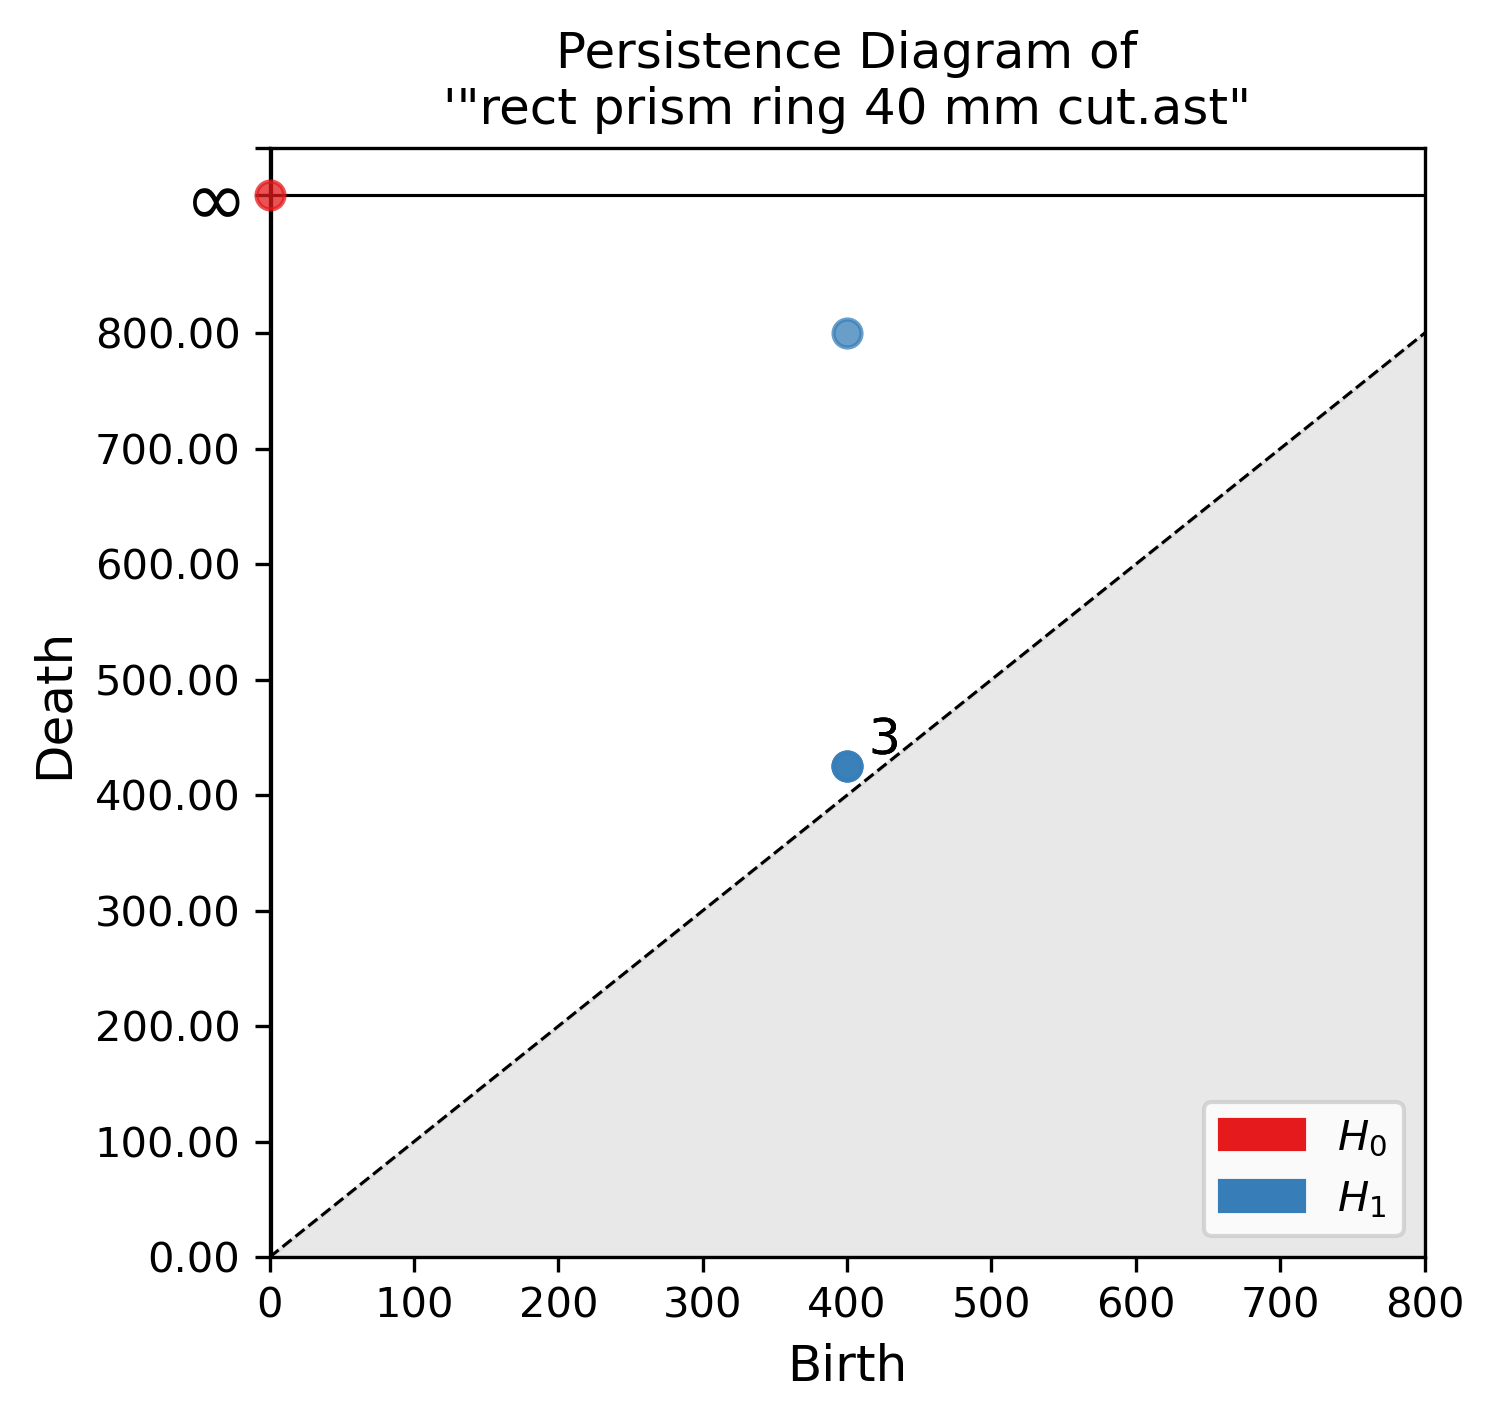
\includegraphics[width=0.18\textwidth]{Final Run, (rect prism ring 40 mm cut) persdia.png} &
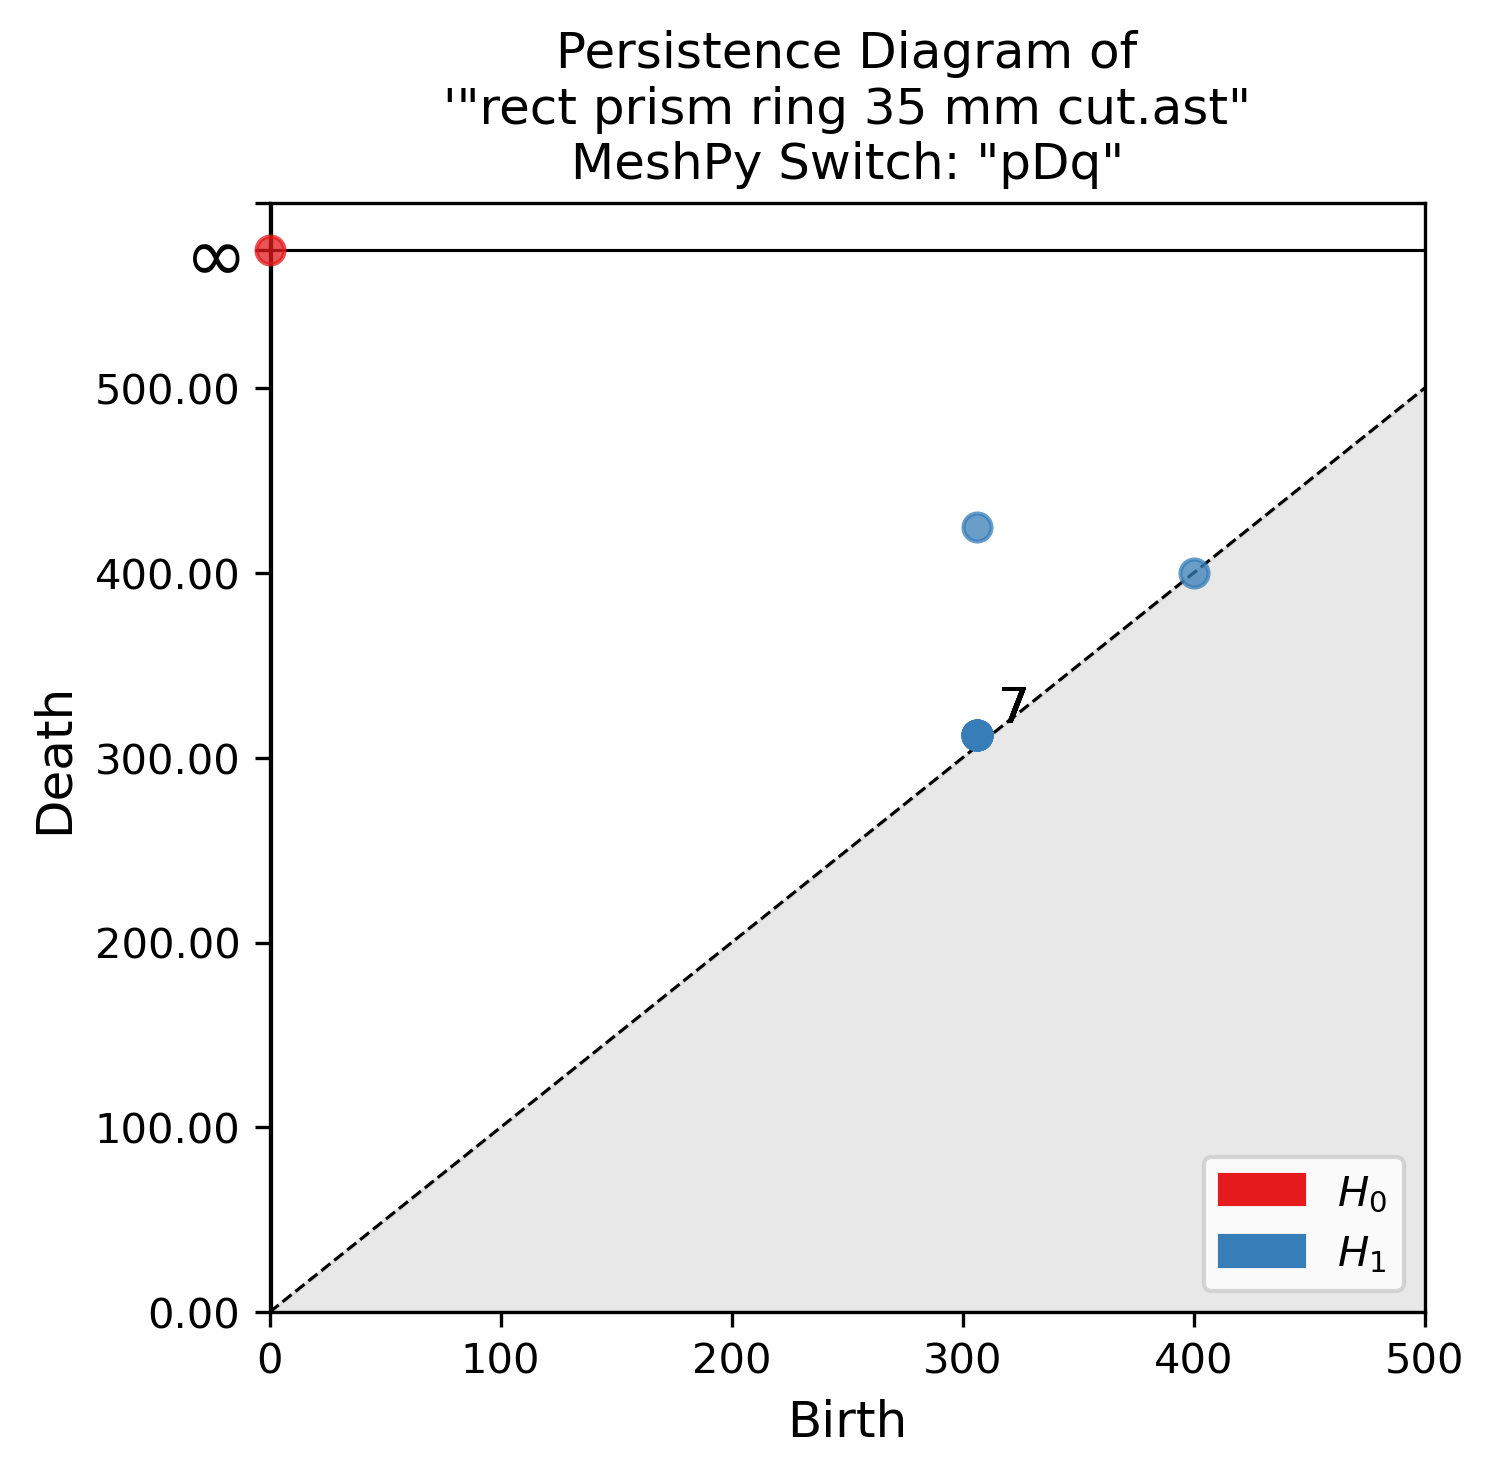
\includegraphics[width=0.18\textwidth]{Final Run, (rect prism ring 35 mm cut) persdia.png} &  
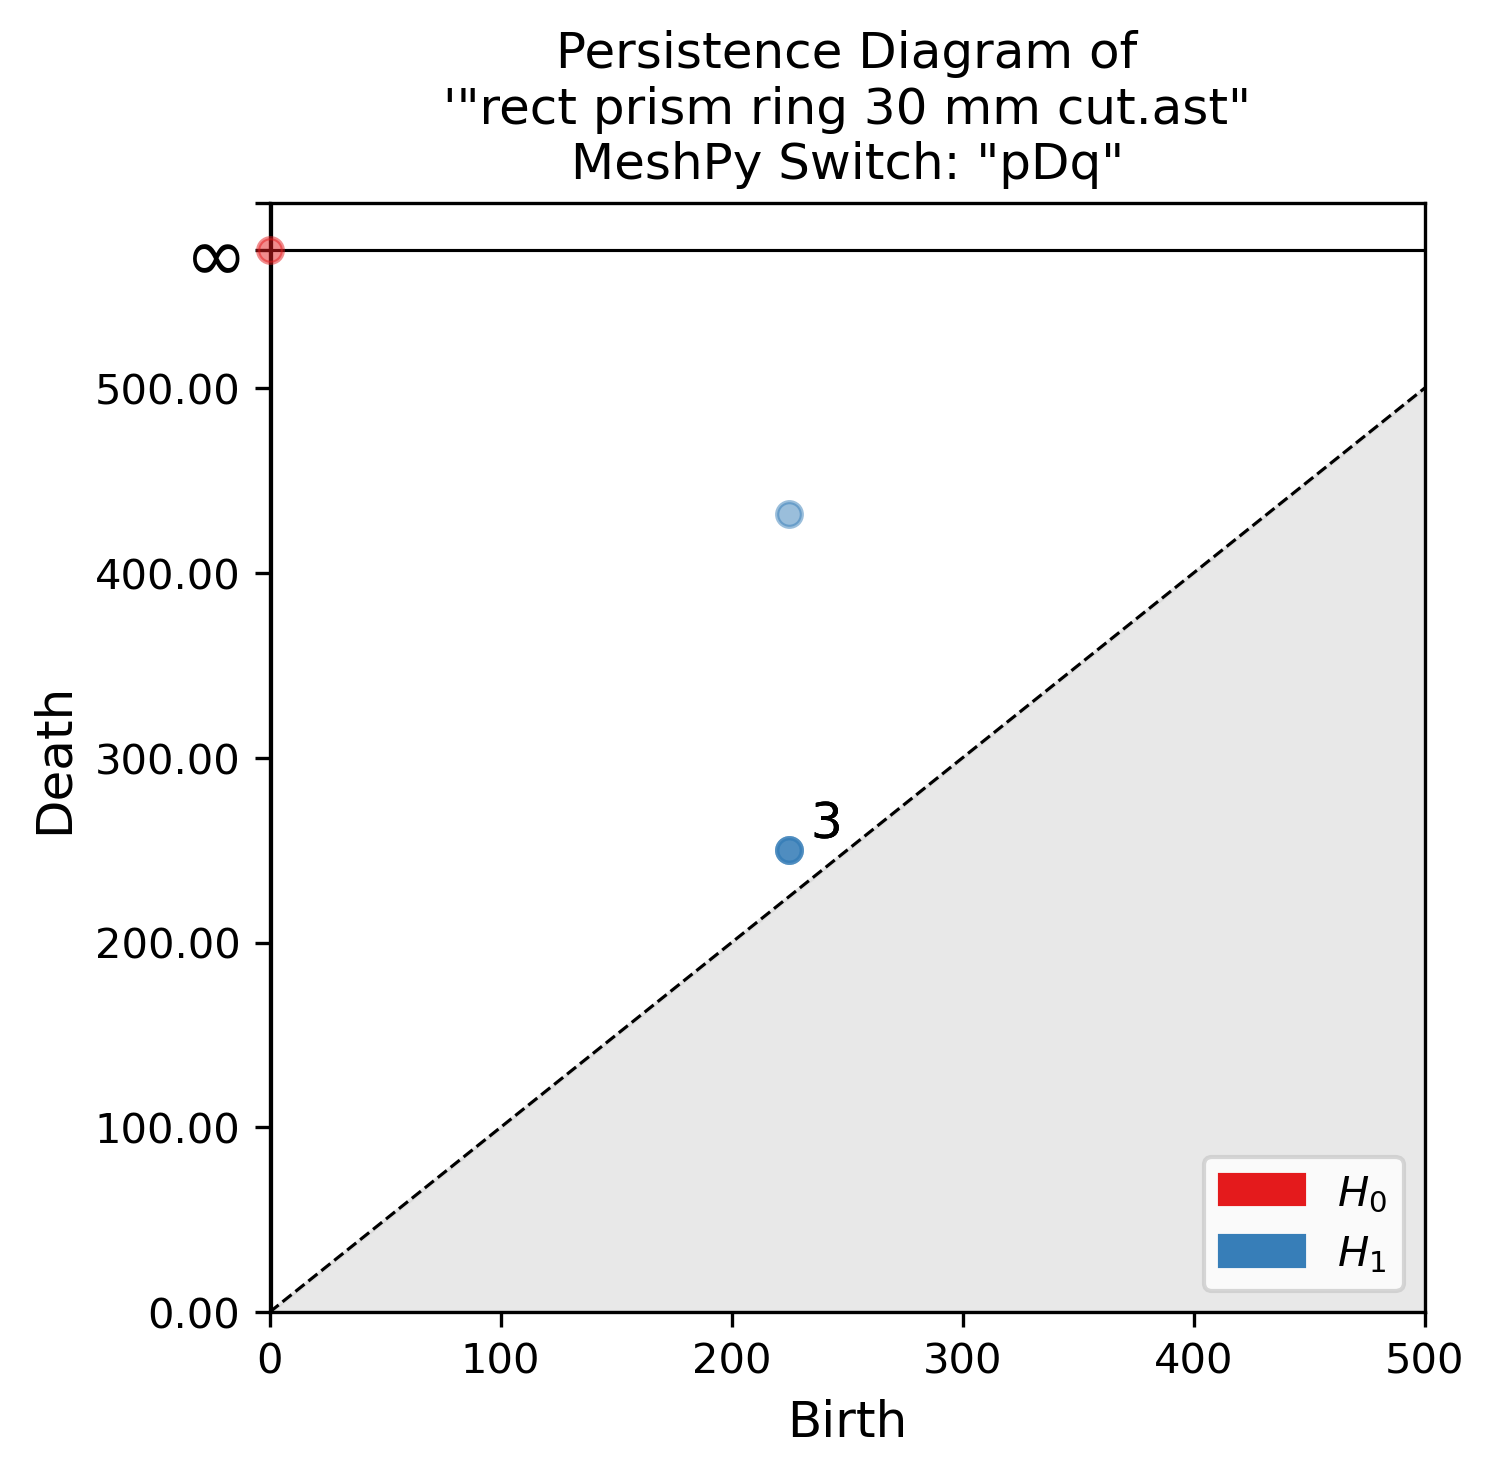
\includegraphics[width=0.18\textwidth]{Final Run, (rect prism ring 30 mm cut) persdia.png} &
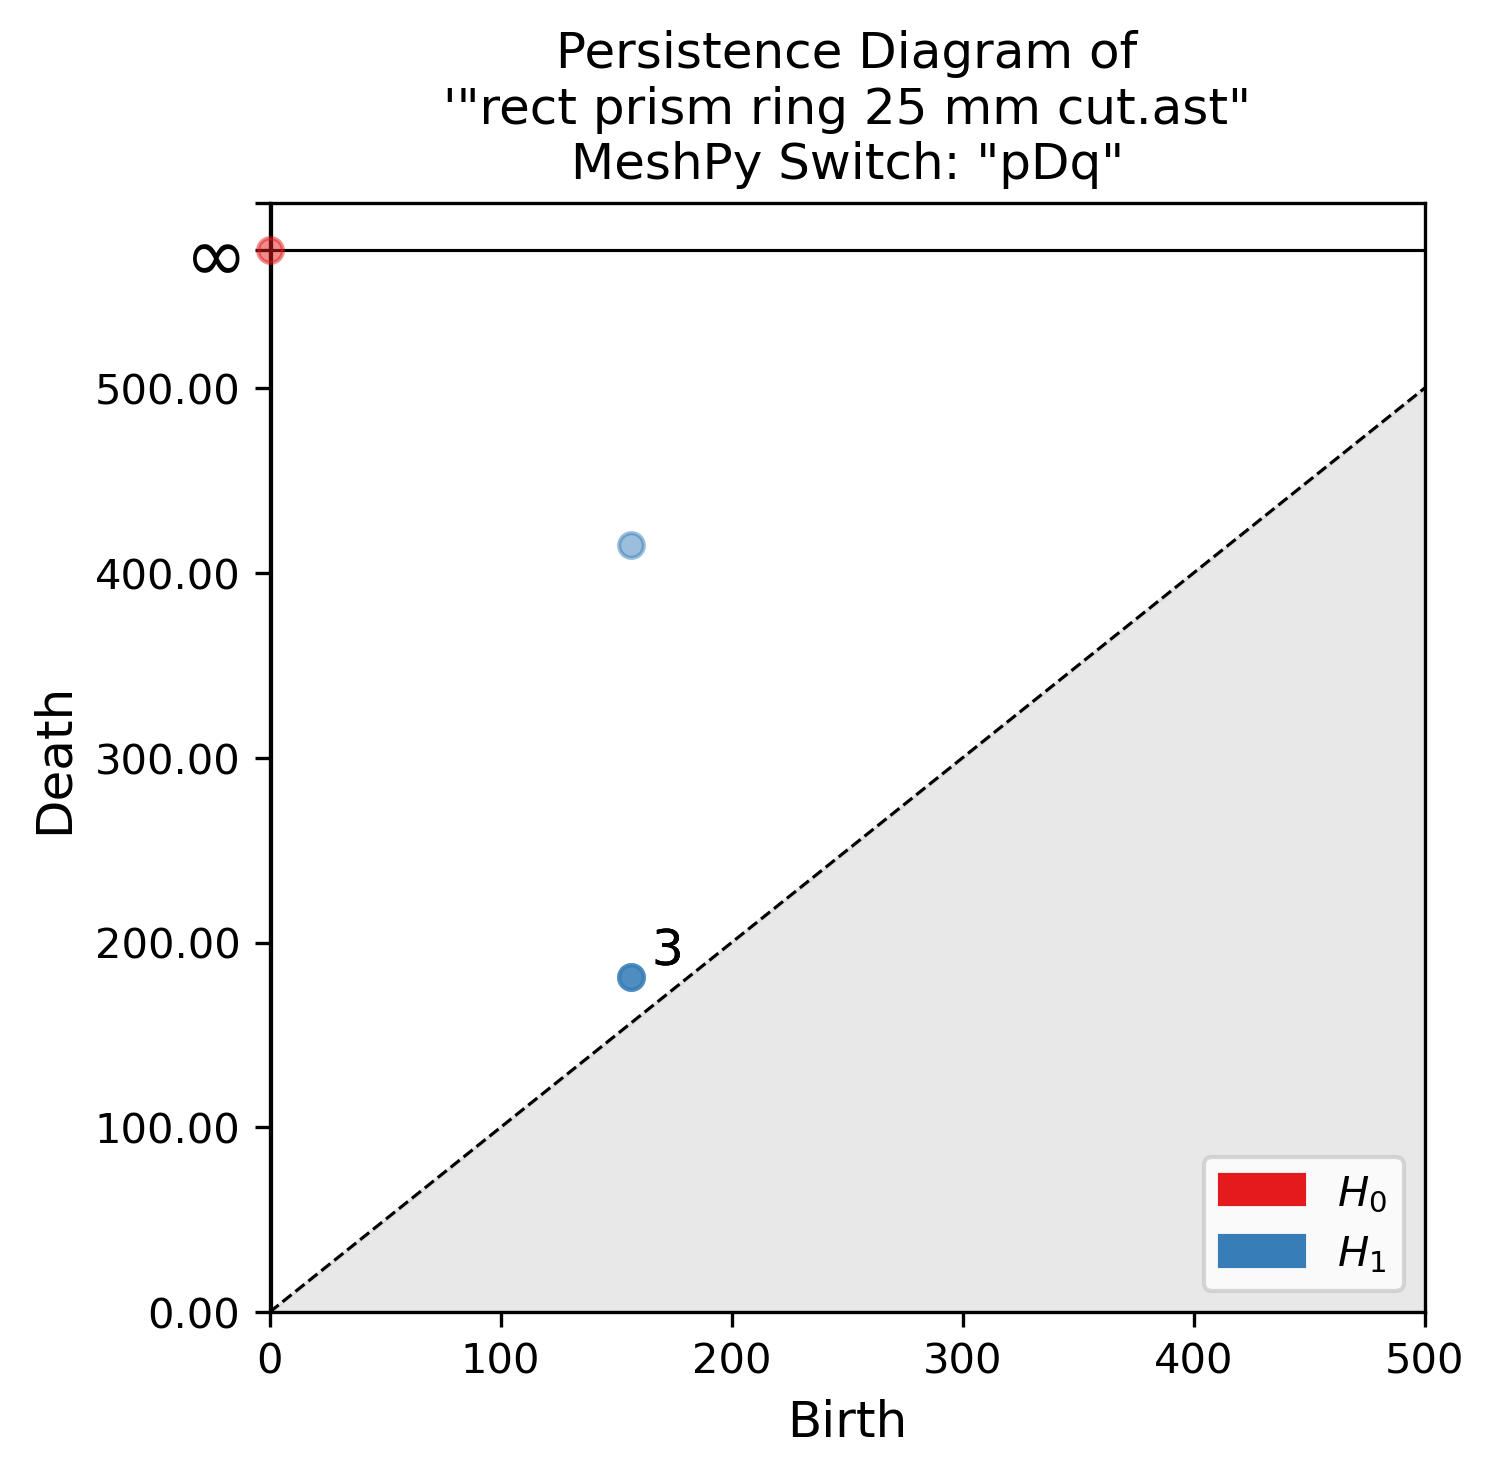
\includegraphics[width=0.18\textwidth]{Final Run, (rect prism ring 25 mm cut) persdia.png} & 
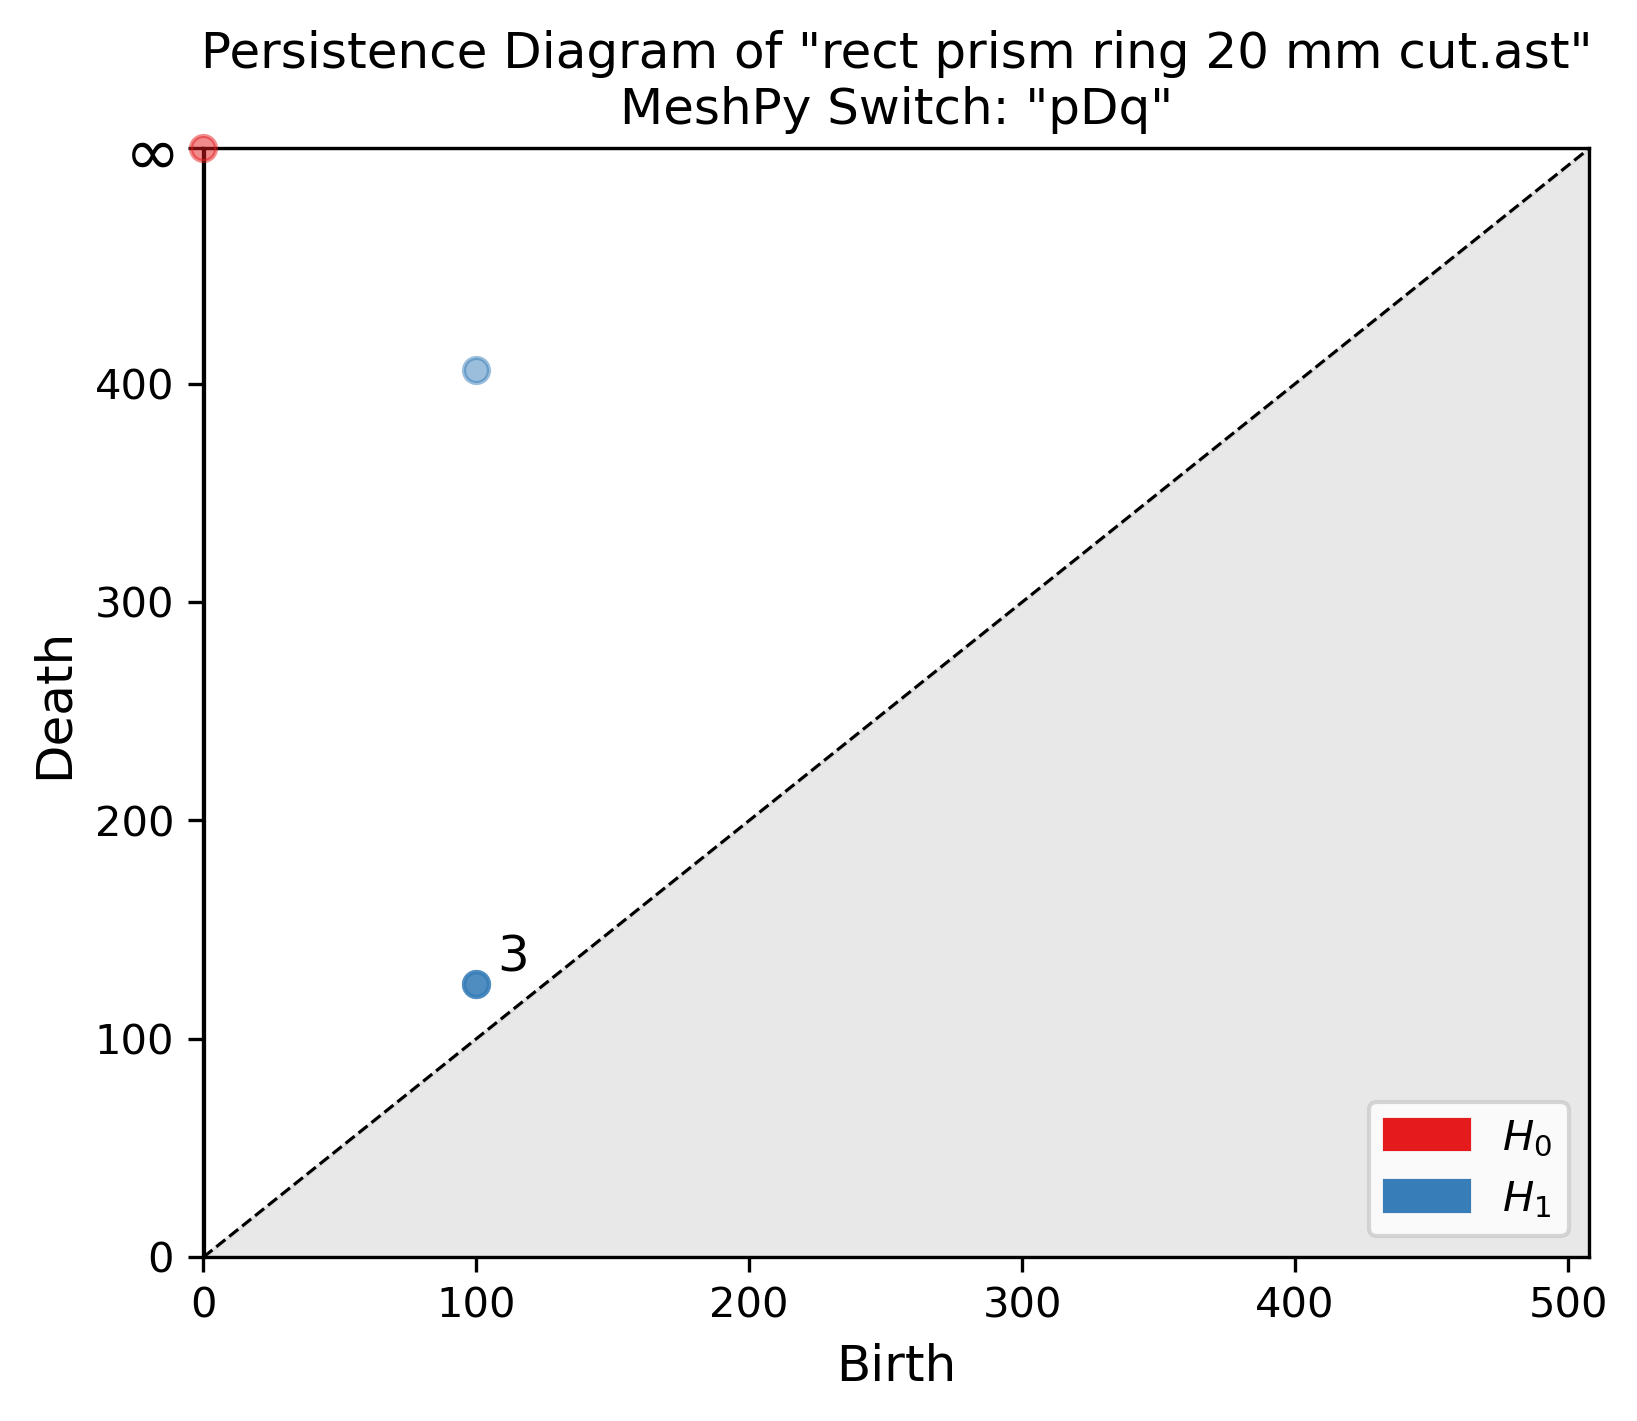
\includegraphics[width=0.18\textwidth]{Final Run, (rect prism ring 20 mm cut) persdia.png} & 
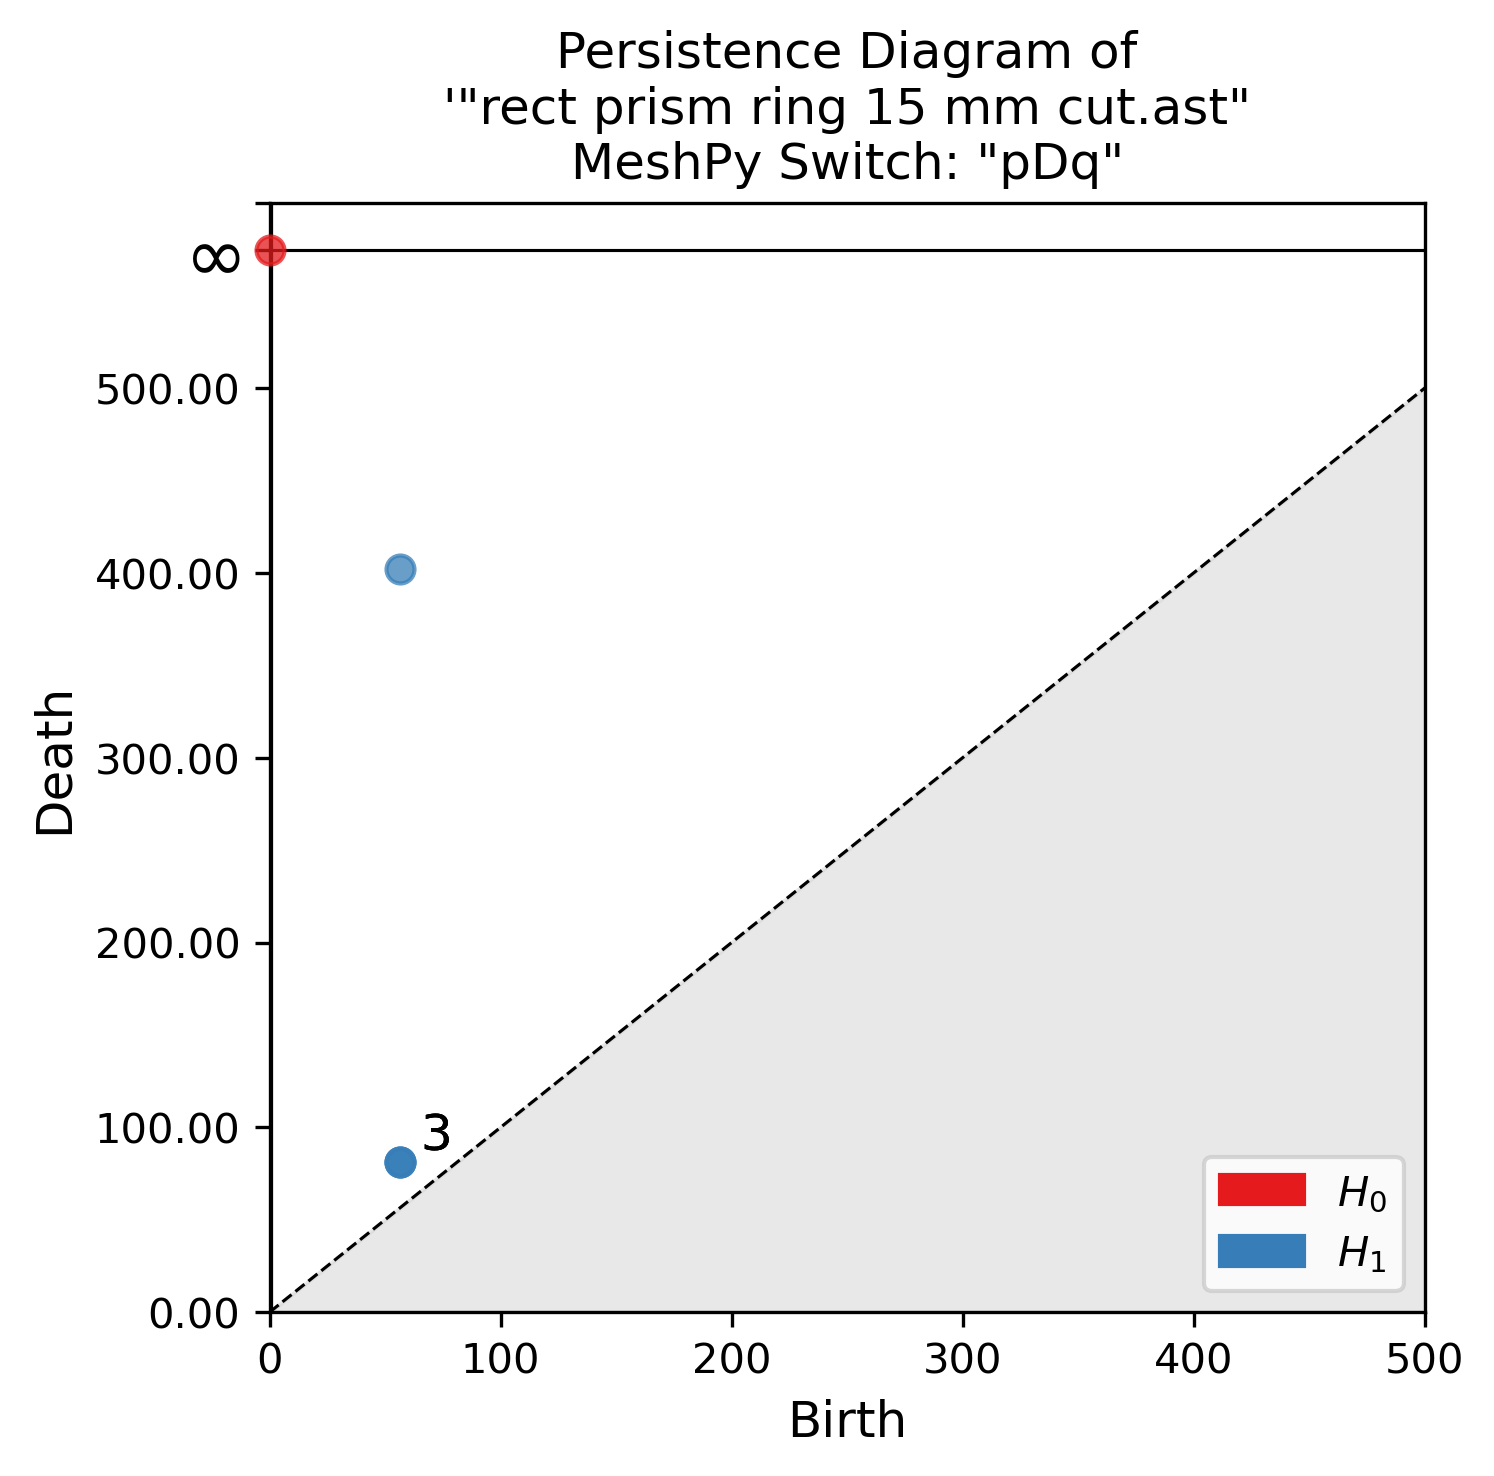
\includegraphics[width=0.18\textwidth]{Final Run, (rect prism ring 15 mm cut) persdia.png} \\
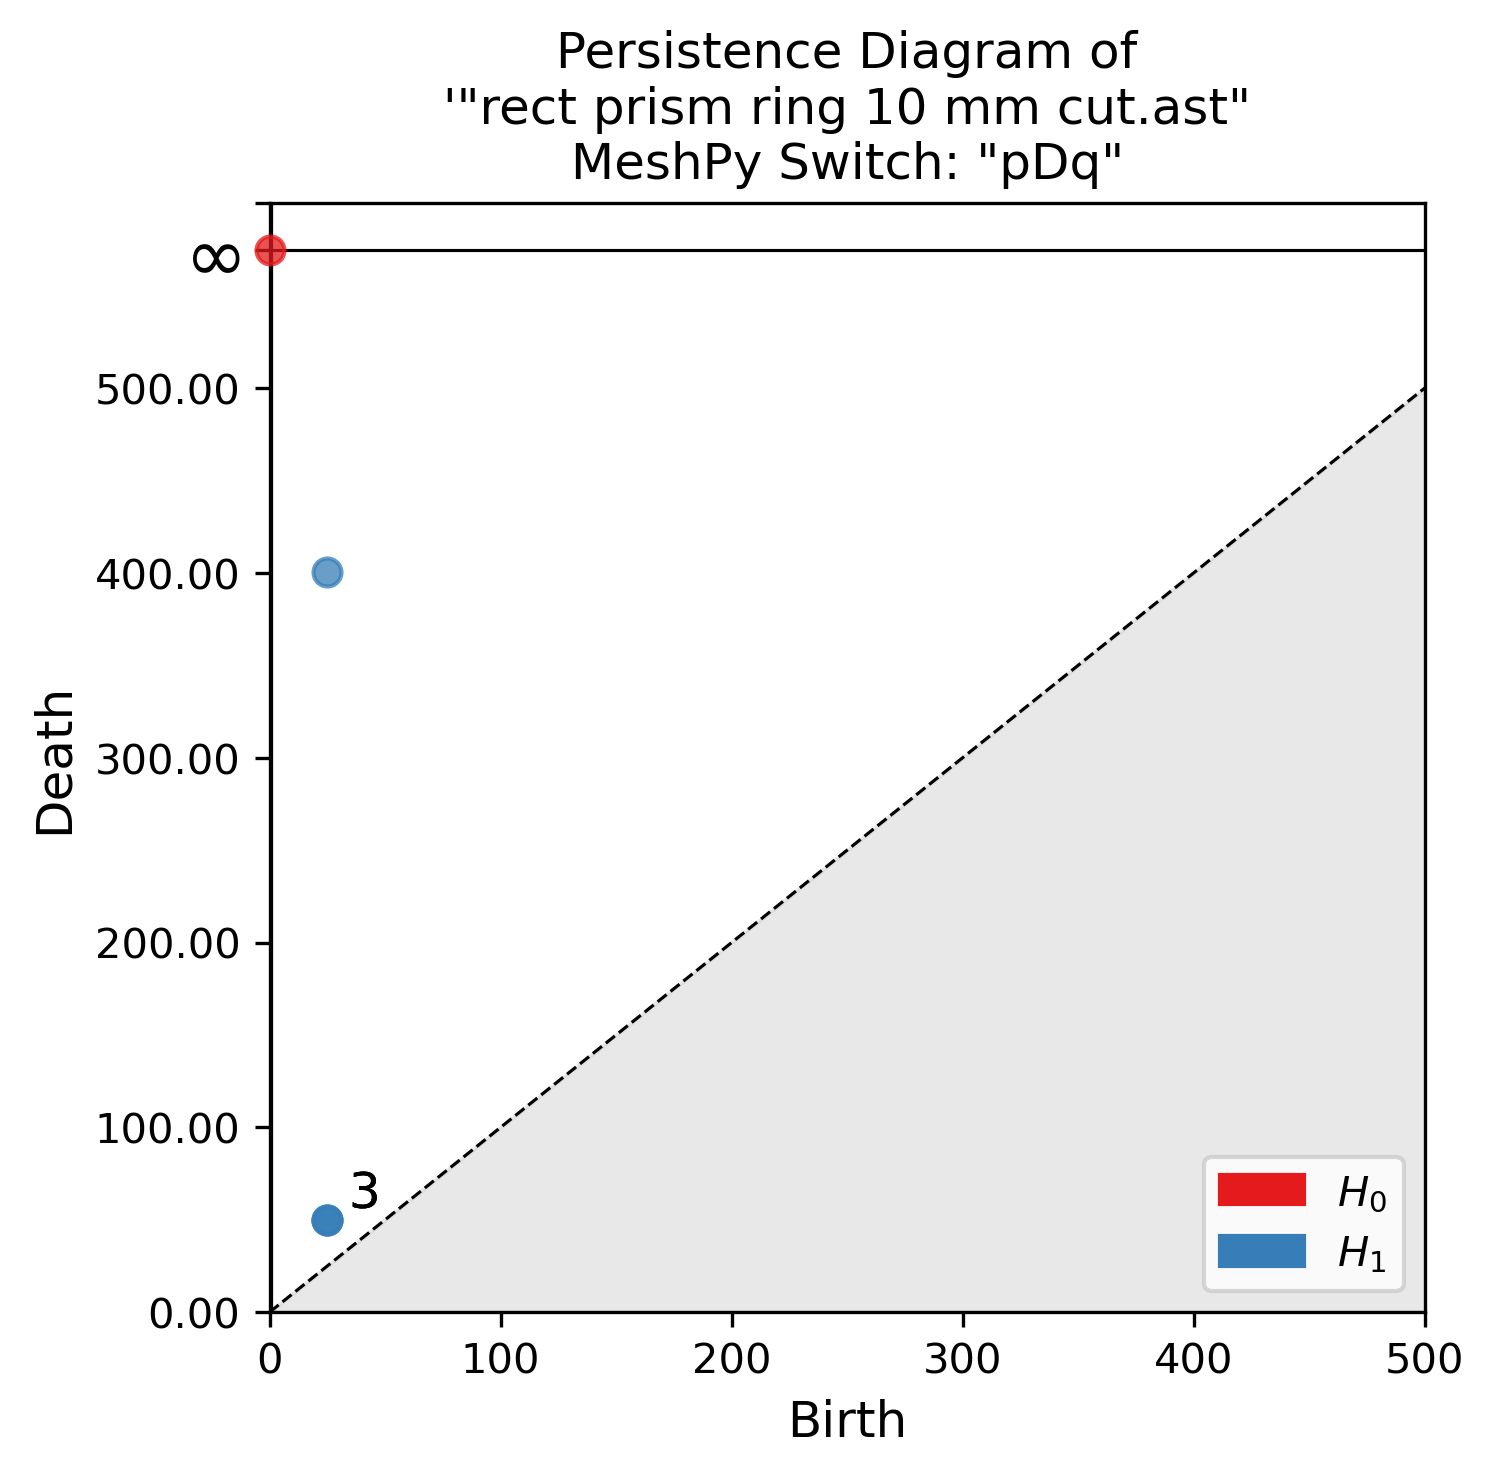
\includegraphics[width=0.18\textwidth]{Final Run, (rect prism ring 10 mm cut) persdia.png} & 
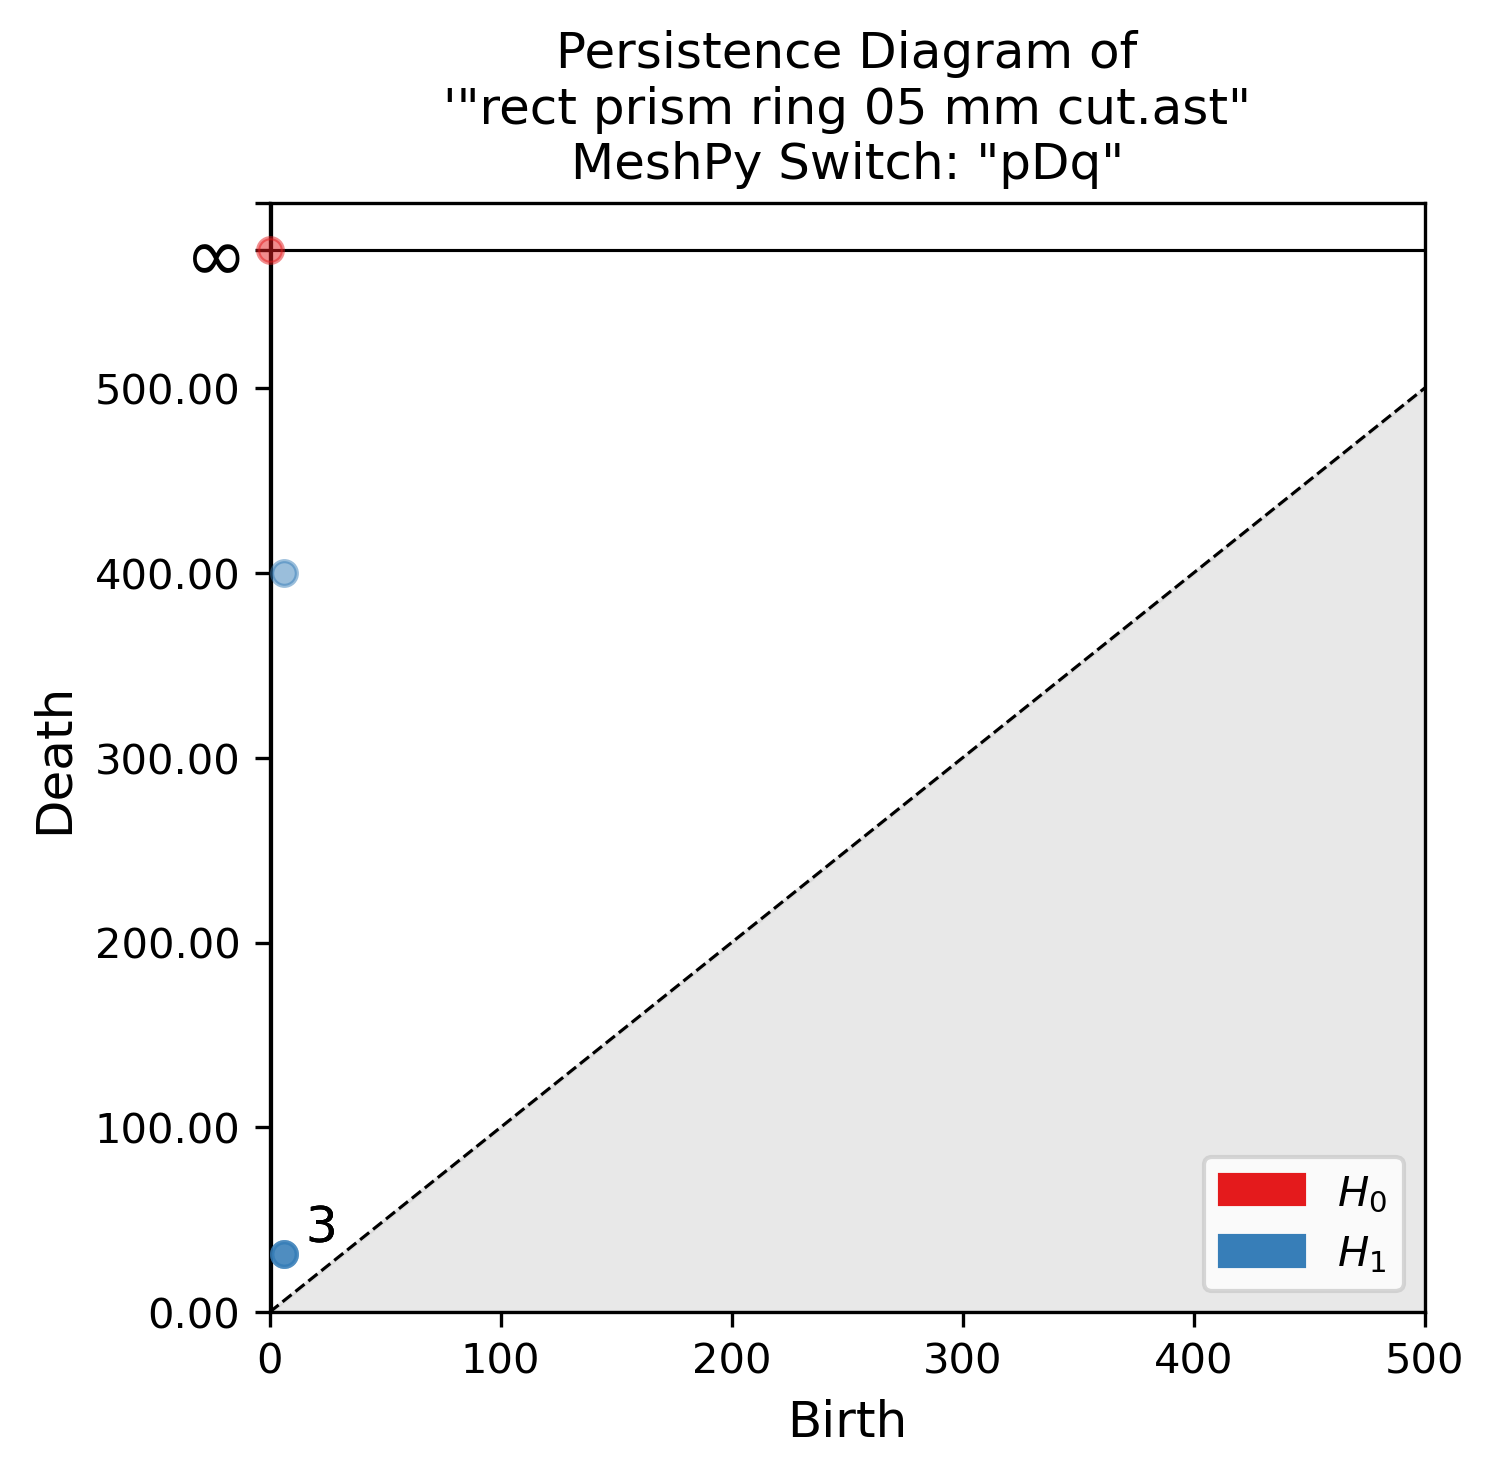
\includegraphics[width=0.18\textwidth]{Final Run, (rect prism ring 05 mm cut) persdia.png} & 
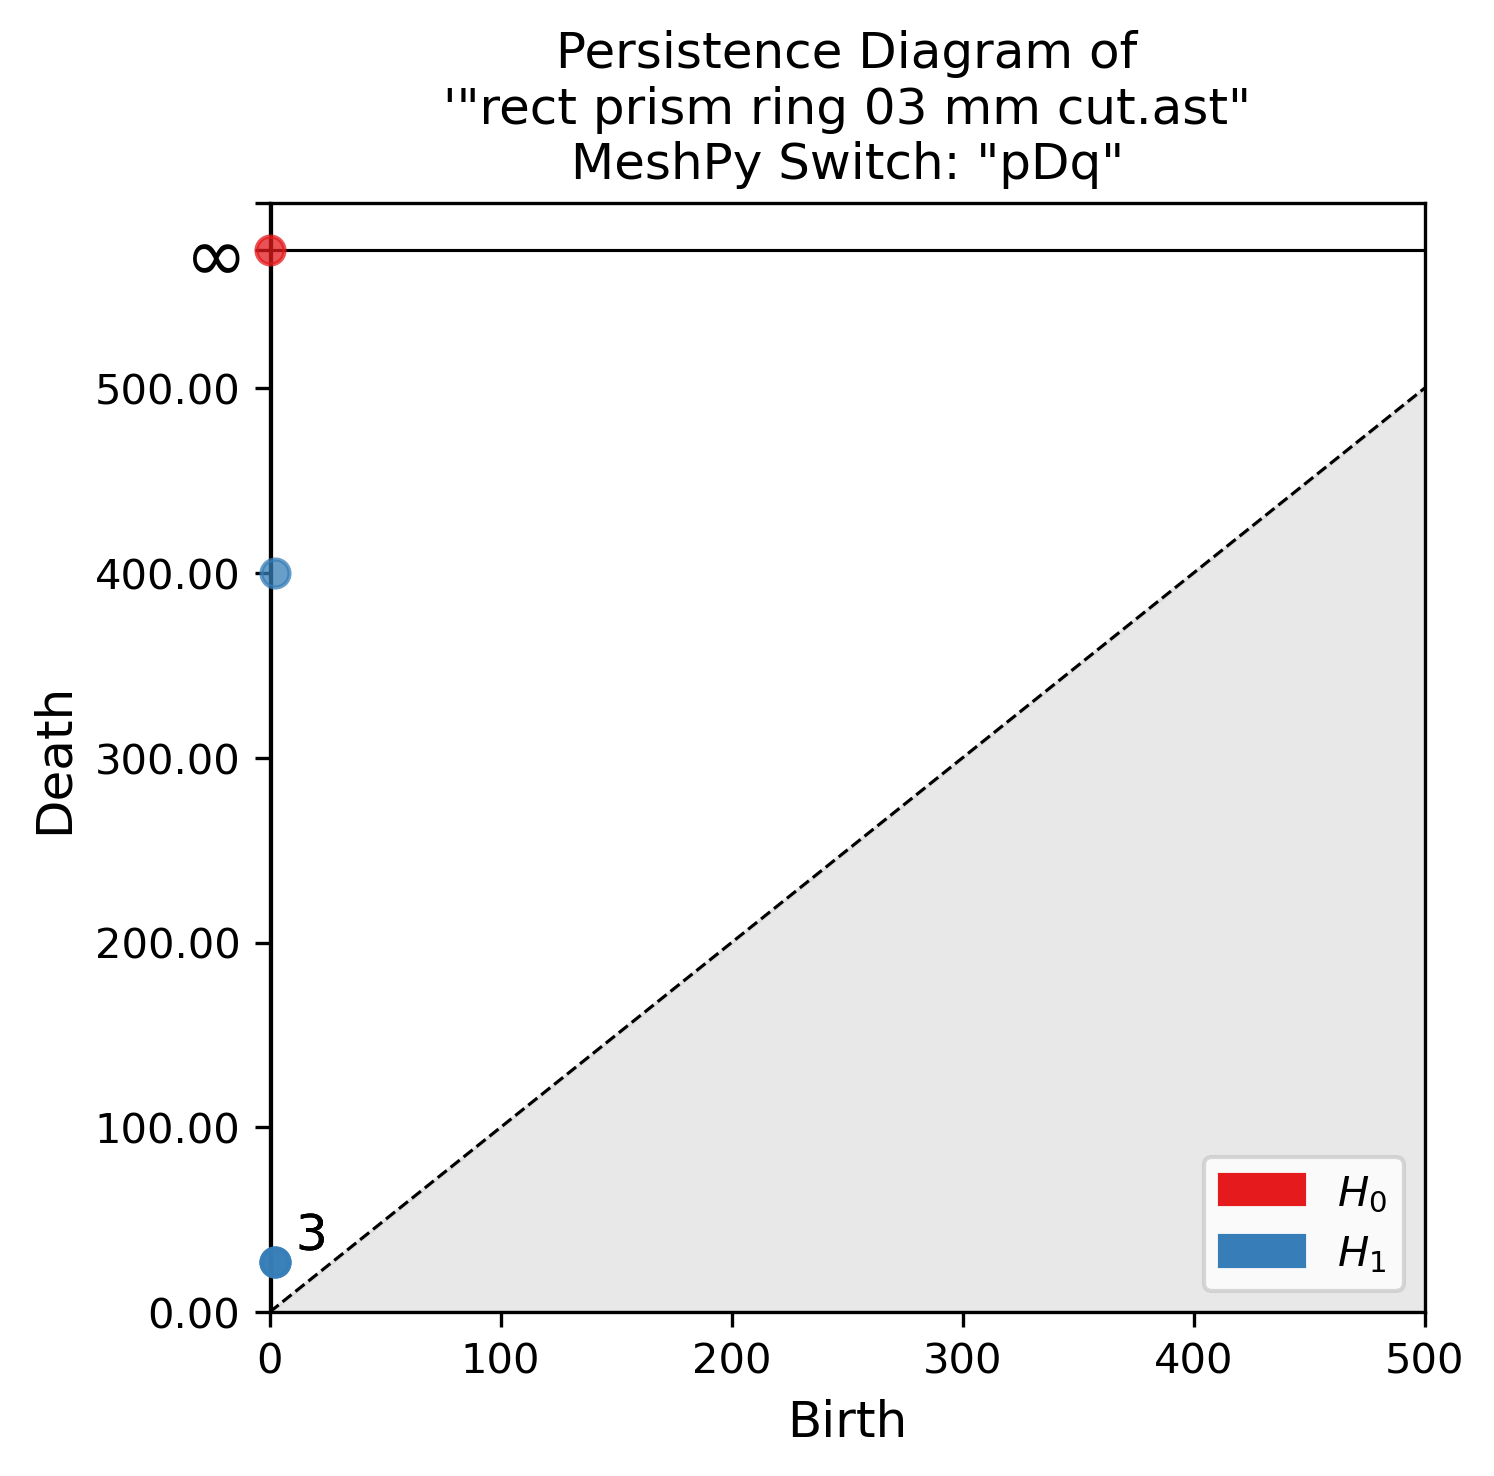
\includegraphics[width=0.18\textwidth]{Final Run, (rect prism ring 03 mm cut) persdia.png} &
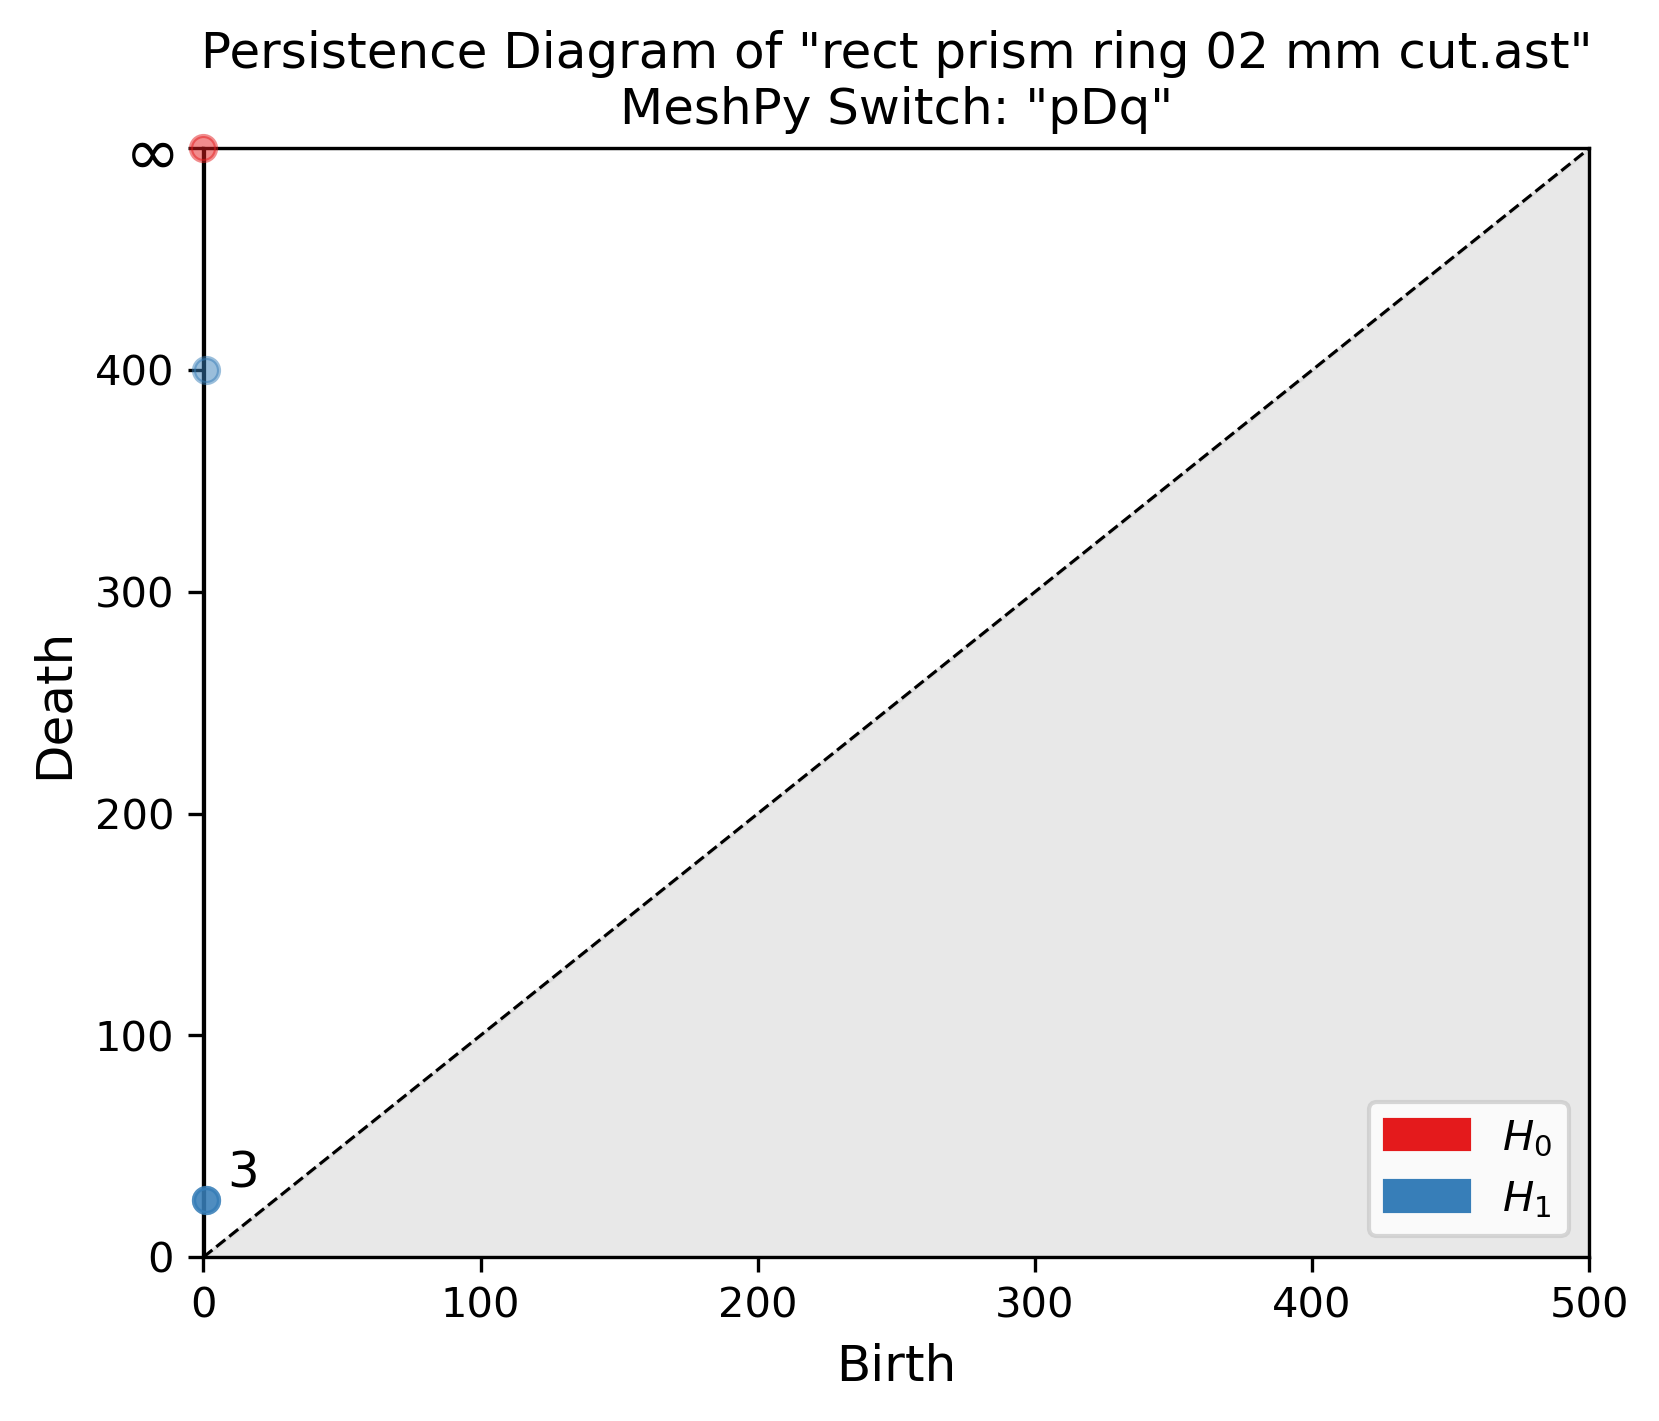
\includegraphics[width=0.18\textwidth]{Final Run, (rect prism ring 02 mm cut) persdia.png} &
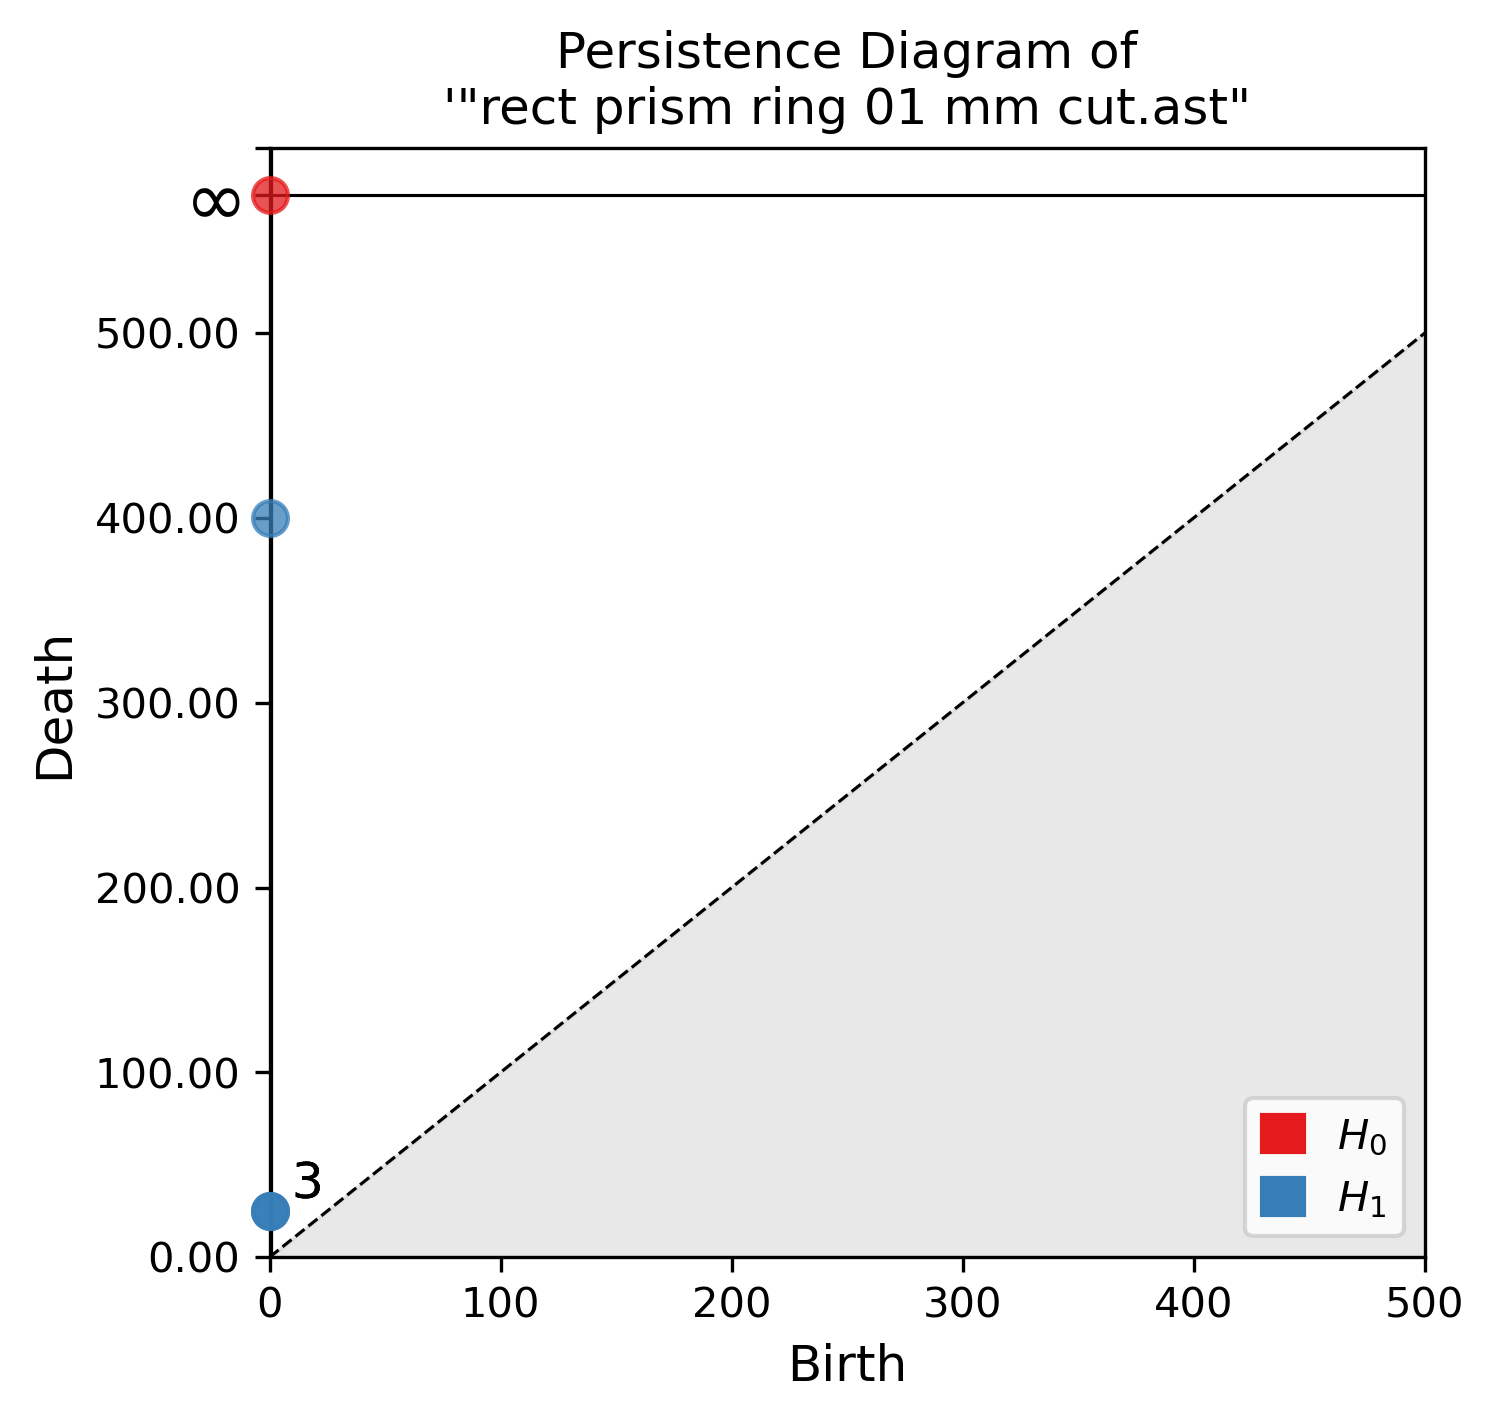
\includegraphics[width=0.18\textwidth]{Final Run, (rect prism ring 01 mm cut) persdia.png} &
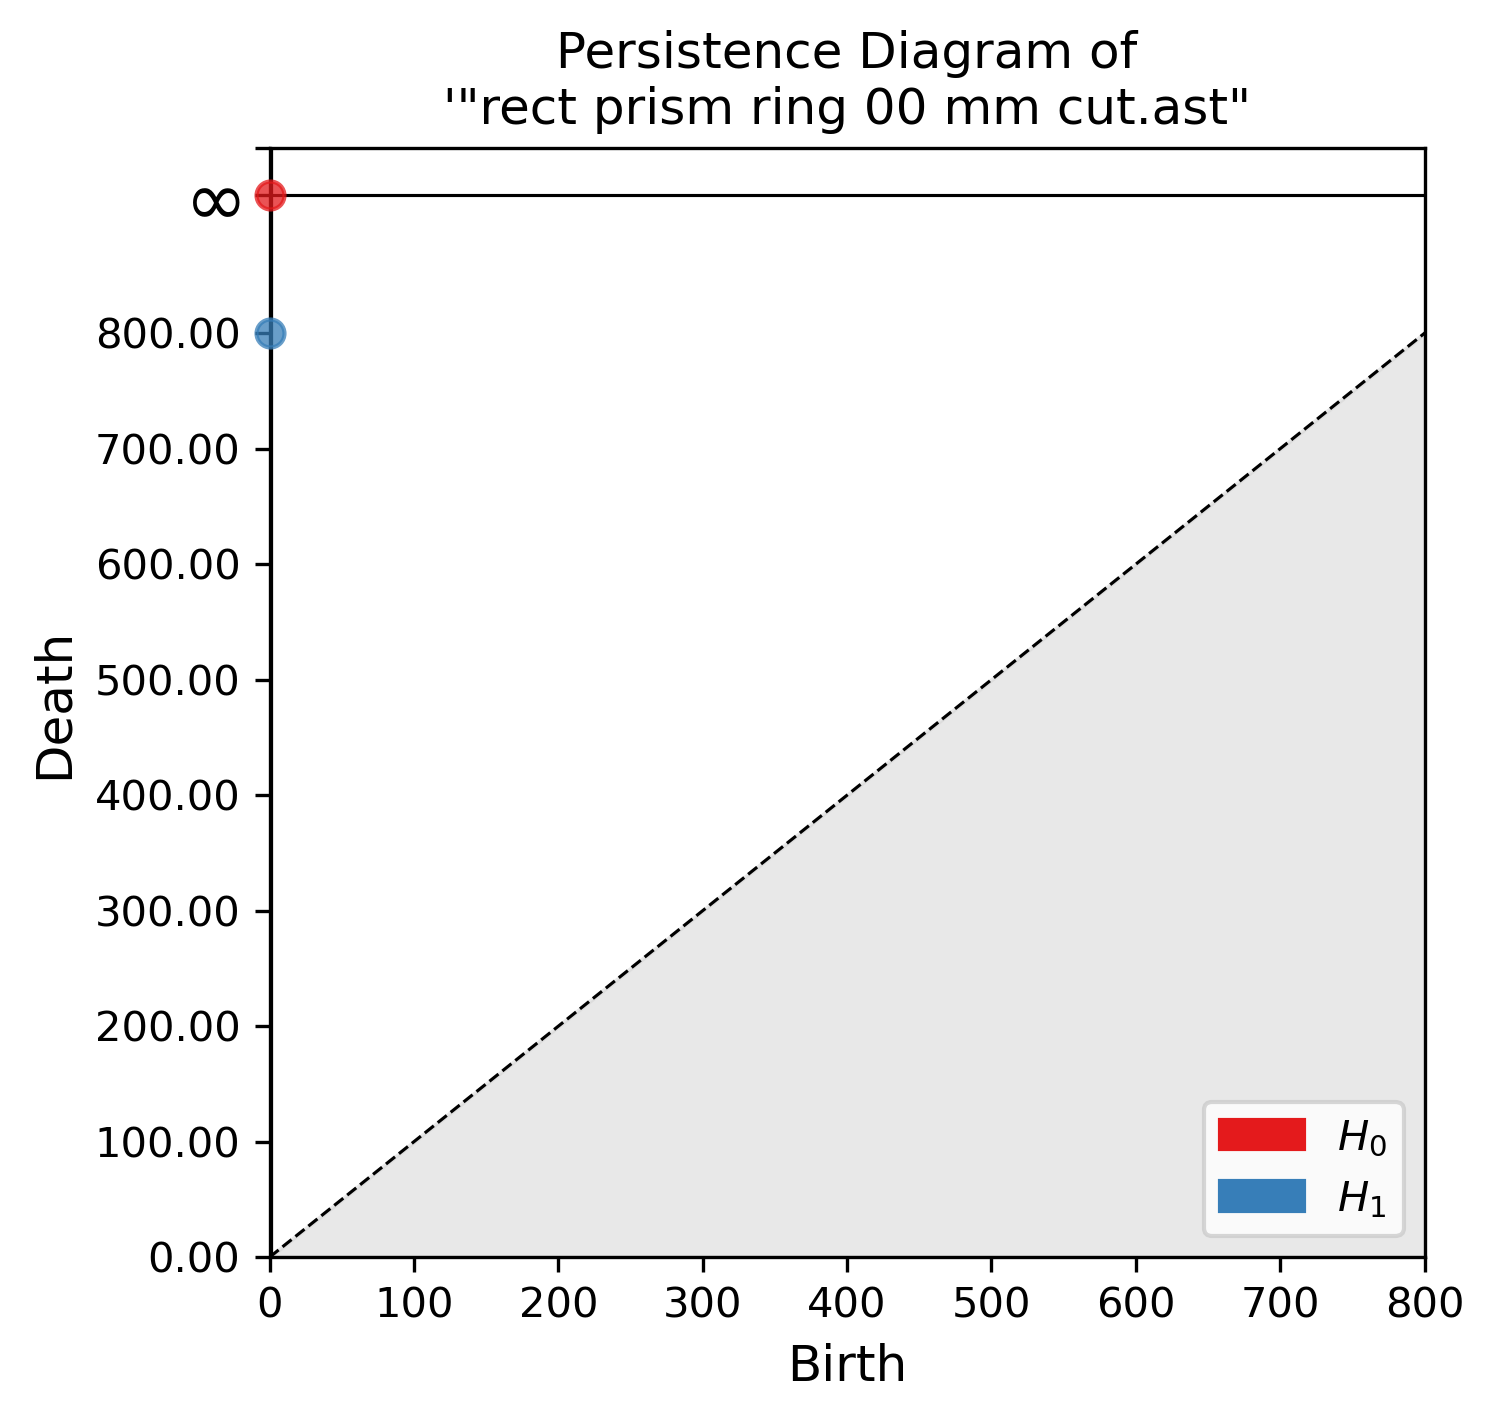
\includegraphics[width=0.18\textwidth]{Final Run, (rect prism ring 00 mm cut) persdia.png} \\
\end{tabular}
\caption{Persistence Diagrams of a rectangular prism ring with a cut that decreases to the original shape.}
\label{fig:rect_prism_ring_persdia_table}
\end{table}
\end{frame}

\section{Conclusion}
\begin{frame}{Conclusion}

\end{frame}

\subsection{Future Work}
\begin{frame}{Future Work}

\end{frame}
\end{document}